\chapter{[Por revisar] Estado del arte}
\label{chapter:estado_arte}

\chapquote{Solo sé que no se nada.}{Sócrates}


En este capítulo se introduce una revisión del estado del arte y del estado de la cuestión en lo que respecta al marco teórico del proyecto que se propone en este \gls{tfm}, así como una descripción sobre los sistemas que existen en el mercado o que han sido reportados en la literatura, los cuales presentan aspectos comunes con la solución propuesta.

\section{Análisis de la situación actual}

    En esta sección, se pone en valor y/o contraste la información introducida en las secciones anteriores, de tal forma que pueda realizarse un análisis del entorno en el que se desarrolla este proyecto, así como también se pueda poner de manifiesto la relevancia y la idoneidad del desarrollo propuesto. 
    
    \subsection{Monitorización mediante dispositivos biométricos}
        \label{sec:estado_arte:biometricos}

        Durante los últimos años se han realizado numerosos experimentos en el ámbito científico con el objetivo de encontrar medidas biométricas que puedan servir de indicadores de algunos de los trastornos de salud mental con medidas biométricas, o bien patrones de comportamiento que también puedan servir de predictor.

        En un estudio comparativo del año 2021 \cite{hickey_smart_2021}, los investigadores realizaron una revisión de los 21 artículos publicados para tratar de identificar las medidas biométricas que permitan identificar depresión, ansiedad y estrés.

        Según este estudio, la \gls{vfc} es una medida muy utilizada para detectar estrés y ansiedad, mejorando su efectividad si se utiliza junto con \glspl{eeg}. Por otra parte, la \gls{eda} se vislumbra como otro buen indicador para el estrés, con la desventaja de su falta de fiabilidad. En cuanto a la depresión, se determinó un uso sistemático de los \glspl{eeg}, pero con dispositivos que no se encuentran a la venta en los mercados.

        En este área de trabajo se puede encontrar al estudio \textit{WESAD} \cite{schmidt_introducing_2018}, del año 2018. En este artículo fue construido un \gls{dataset} para la detección de estrés con datos de 15 voluntarios, mediante un dispositivo colocado en el pecho y otro en la muñeca. El primero de ellos se encargó de recoger datos de \glspl{ecg}, respiración y de movimiento (mediante acelerómetros), mientras que el segundo de ellos recogía datos de temperatura corporal, \gls{eda}, \gls{bvp} y nuevamente de movimiento mediante acelerómetros.

        Con estos datos se planteó un problema de clasificación binaria (estrés o ausencia del mismo) mediante diversos algoritmos (árboles de decisión, \textit{random forest}, k-vecinos más cercanos o \textit{KNN}), obteniéndose precisiones entre el 69\% y el 86\% si se utilizaban los datos del dispositivo de pecho y entre el 67\% y el 88\% para los correspondientes a la muñeca. Si el lector lo desea, puede consultar en \cite{schmidt_introducing_2018} las tablas del estudio donde se detalla la precisión por cada algoritmo y dato utilizado.

        En una línea similar el artículo \textit{PASS} \cite{parent_pass_2020} del año 2020 también plantea la construcción de un \gls{dataset} para la detección de estrés con datos de 48 participantes. La principal diferencia con el estudio anterior es el establecimiento de un entorno controlados para provocar cambios en los niveles de estrés a través de videojuegos; mientras que los datos recolectados son fundamentalmente los mismos: \glspl{ecg}, \gls{eda}, respiración, temperatura corporal y \glspl{eeg}.

    \subsection{Monitorización mediante datos de smartphones}
        \label{sec:estado_arte:smartphone}

        Los estudios anteriores construyeron \glspl{dataset} en condiciones de laboratorio, utilizando \glspl{invasiva} para la monitorización de las constantes de los voluntarios. En contraposición a estas mediciones, existen otros estudios que apuestan por un enfoque basados en \glspl{no-invasiva}, en este caso mediante \glspl{wearable} o con \glspl{smartphone}, siendo procedimientos más cercanos a los usuarios en su día a día. En este ámbito se puede encontrar los proyectos \textit{DemonicSalmon} \cite{boukhechba_demonicsalmon_2018} y \textit{StudentLife} \cite{rui_studentlife_2014}.

        \textit{DemonicSalmon} es un proyecto realizado en 2018, en el cual se monitorizó la salud mental diariamente de 72 estudiantes en un intervalo de dos semanas. En particular, se estudió la ansiedad social y los síntomas de depresión, obteniéndose correlaciones significativas con patrones de movilidad (detectados mediante GPS), niveles de actividad (medidos mediante acelerómetros) y patrones de comunicación (obtenidos mediante registros de llamadas y SMS) \cite{boukhechba_demonicsalmon_2018}. Los datos obtenidos fueron recogidos en un \gls{dataset} para su uso en trabajos futuros.

        El segundo de ellos, \textit{StudentLife}, se trata del más veterano de ellos, ya que data de 2014. Este artículo, entre otras cuestiones, estudia la salud mental en el marco de una clase de 48 estudiantes en un periodo de 10 semanas. Entre otras medidas, se estudiaron niveles de estrés, depresión y soledad, estando dichos niveles caracterizados por los cuestionarios PSS-10, PHQ-9 y UCLA-20 respectivamente; realizados antes y después del periodo de estudio.
        
        A partir de los \glspl{smartphone}, los investigadores realizaron un profundo trabajo de extracción de datos, recogiendo datos de llamadas y SMS, inferiendo perfiles de actividad física, duración de sueño y patrones de movilidad, entre otros. Asimismo, los estudiantes realizaron una serie de cuestionarios diarios durante el proceso.

        Con estos datos, se obtuvieron entre otras las siguientes correlaciones y asociaciones, detalladas en \cite{rui_studentlife_2014}:

        \begin{itemize}
            \item Estrés con la duración de las conversaciones y la duración del sueño.
            \item Depresión con la duración y frecuencia de las conversaciones, coubicación\footnote{El artículo lo define como \textit{el número de dispositivos Bluetooh co-ubicados}, lo que se podría entender como la cantidad de personas que están junto al usuario en cada momento.} y la duración de sueño.
            \item Sentimiento de soledad con la actividad física y la movilidad del usuario.
        \end{itemize}
    
    \subsection{Cuidado del bienestar emocional mediante aplicaciones móviles}
        \label{sec:estado_arte:apps}

        Fuera del ámbito académico, la creciente digitalización de la sociedad impulsada por las aplicaciones móviles también se ha reflejado en el campo de la salud mental en los últimos años, con una gran variedad de iniciativas por parte de numerosos actores.

        Se puede considerar en primer lugar los esfuerzos \textit{oficiales} de Google y Apple para añadir nuevas funcionalidades a sus sistemas operativos, Android e iOS, respectivamente. En el caso de Google se trata de un componente nuevo \textit{Bienestar Digital} \cite{android_bienestar_nodate}, mientras que Apple decidió ampliar la funcionalidad de su aplicación \textit{Salud} \cite{apple_newsroom_apple_2023}.
        
        La herramienta \textit{Bienestar Digital}, incluida por defecto en las nuevas versiones de Android, permite, entre otras funciones, establecer un modo descanso en el que no se reciben notificaciones; otro modo denominado \textit{sin distracciones} que pone temporalmente en pausa aplicaciones escogidas por el usuario, visualizar mediante \glspl{widget} y paneles estadísticas relacionadas con el uso de cada aplicación o la posibilidad de limitar el tiempo de uso de ciertas aplicaciones. En la Figura \ref{fig:estado_arte:bienestar_digital} se pueden ver ejemplos tomados desde el móvil del autor.

        \begin{figure}[h]
            \begin{subfigure}[t]{0.48\textwidth}
                \includegraphics[width=1\linewidth]{figures/Estadísticas uso.jpg}
            \end{subfigure}
            \hfill
            \begin{subfigure}[t]{0.49\textwidth}
                \includegraphics[width=1\linewidth]{figures/Limitador de aplicación.jpg}
            \end{subfigure}
            \caption{Ejemplos de las funciones de \textit{Bienestar Digital}}
            \label{fig:estado_arte:bienestar_digital}
        \end{figure}

        Por otra parte, en la versión 17 de iOS, fueron incorporadas a la aplicación \textit{Salud} características para que los usuarios reflexionaran sobre su estado de bienestar emocional, elementos de evaluación de ansiedad y depresión usados en los centros sanitarios, o estadísticas relacionadas con la salud visual. Nuevamente, se presentan algunos ejemplos en la Figura \ref{fig:estado_arte:ios_salud}.

        \begin{figure}[h]
            \begin{subfigure}[t]{0.49\textwidth}
                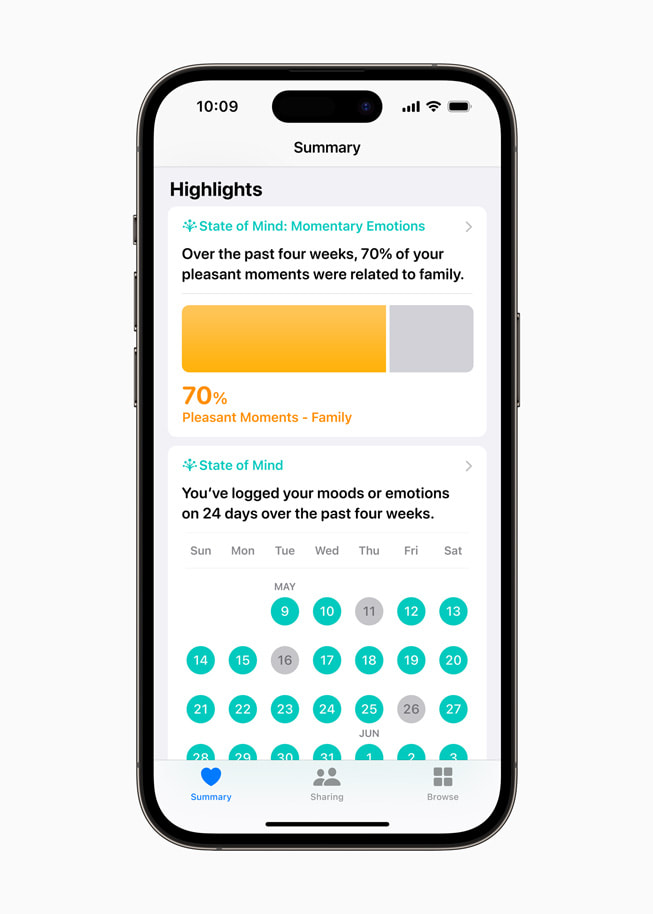
\includegraphics[width=1\linewidth]{figures/ios seguimiento bienestar emocional.jpg}
            \end{subfigure}
            \hfill
            \begin{subfigure}[t]{0.49\textwidth}
                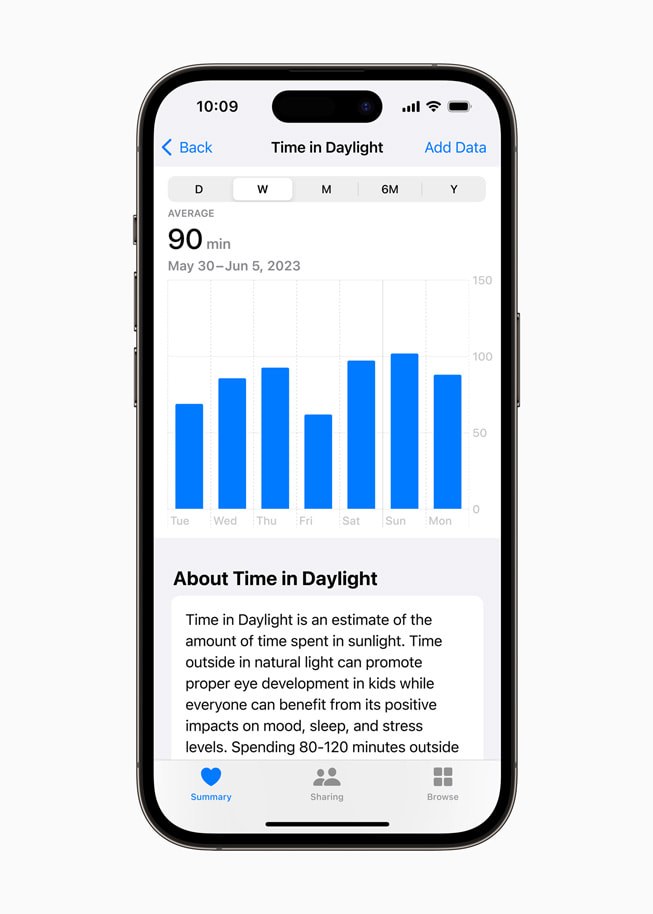
\includegraphics[width=1\linewidth]{figures/ios salud visual.jpg}
            \end{subfigure}
            \caption[Ejemplos de las funciones de bienestar de la aplicación \textit{Salud} de iOS]{Ejemplos de las funciones de bienestar de la aplicación \textit{Salud} de iOS, extraídos de \cite{apple_newsroom_apple_2023}.}
            \label{fig:estado_arte:ios_salud}
        \end{figure}

        En cuanto a las aplicaciones específicas desarrolladas por terceros, se trata de un mercado con gran proyección. El uso de estas aplicaciones creció, entre 2019 y 2021, un 54,6\% \cite{bejerano_lado_2023}, a la vez que el mercado global de estas apps se estimó en un valor aproximado de 6.200 millones de dólares en 2023; proyectándose un crecimiento incremento anual del 15,8\% hasta en 2030 según un análisis de \textit{Grand View Research} \cite{grand_view_research_mental_nodate}.
        
        Dentro de estas aplicaciones se pueden hallar varios enfoques. Por una parte existen plataformas como \textit{BetterHelp} o \textit{Talkspace}, las cuales hacen de intermediarios de usuarios con terapeutas, digitalizando el acceso al tratamiento. Otras como \textit{Happify} no recurren a profesionales y exploran el ámbito de la gamificación, incluyendo actividades y juegos para mejorar el estado de ánimo del usuario y que este tome un rol más activo. 
        
        Por otra parte, el planteamiento que se observa más común es el de aplicaciones como \textit{Calm}, \textit{Yana} o \textit{Headspace}; las cuales se caracterizan por presentar meditaciones, música o ejercicios al usuario para reducir sus niveles, generalmente, de estrés \cite{modglin_5_2023} \cite{pepinosa_cinco_2023}. Para el acceso al contenido normalmente el usuario debe suscribirse, bien mensualmente o anualmente. 

        Estas aplicaciones presentan la ventaja de poder ser utilizadas en cualquier momento, a la vez que su precio suele ser notablemente inferior al coste de un tratamiento con un especialista. Suscripciones anuales como la de \textit{Calm} cuestan en torno a 65 euros anuales \cite{modglin_5_2023}, mientras que el coste de una consulta de una hora con un psicólogo asciende de media a 52 euros \cite{garcia_santos_boom_2023}. No obstante, el precio de una consulta no muestra el trabajo previo que realiza el profesional para preparar la sesión, ni tampoco muestra la diferencia en la atención al paciente.

        Sin embargo, las aplicaciones tienen una serie de desventajas claras. En primer lugar, para garantizar el rigor científico del contenido ofrecido se necesita que en su desarrollo trabajen profesionales especializados en salud mental, hecho que no suele reflejarse en la información de dichas aplicaciones. Asimismo, casos como el de \textit{Headspace}, una aplicación con más de 60 millones de usuarios, que fue creada por un \textit{``un monje budista tibetano y titulado en Artes Circenses en el Conservatorio de Danza y Teatro de Londres''} \cite{garcia_santos_boom_2023}, siembran ciertas dudas de su rigurosidad científica.
        
        En esta línea de trabajo se han realizado algunos trabajos científicos, debido a la popularidad de estas aplicaciones y su influencia en la salud mental en la sociedad. Según un análisis realizado en 2019 a 293 aplicaciones \cite{marshall_digital_2019}, solo el 3,41\% de las mismas presentaban pruebas científicas de su eficacia. \textit{``De estas 10 aplicaciones, sólo en tres casos la investigación era independiente; es decir, había sido realizada por una institución que no participaba en el desarrollo de la app''} \cite{garcia_santos_boom_2023}.

        Por otra parte, existen fundadas preocupaciones sobre la privacidad de dichas aplicaciones. Según un análisis de la Fundación Mozilla a 37 aplicaciones \cite{mozilla_foundation_privacidad_nodate}, a fecha de junio de 2024 22 de ellas fueron marcadas con la etiqueta \textit{privacidad no incluida}. Asimismo, se han reportado faltas de consentimiento para tratar datos confidenciales, ausencia de transparencia en los procesos o incluso, transcripciones de los chats entre los terapeutas y los usuarios. En el caso de \textit{Talkspace}, según dos ex-empleados \textit{``los científicos de datos de Talkspace compartían frases de estas transcripciones con el equipo de marketing para personalizar la publicidad de los usuarios''} \cite{bejerano_lado_2023}.
        
        En general, actualmente se pueden observar numerosas objeciones a estas aplicaciones tanto sobre su calidad como a la privacidad de los datos tratados, más teniendo en cuenta el impacto que pueden tener sobre la salud de las personas.

\section{Contribución de la solución propuesta}

    En este apartado se introducen las ideas principales que distinguen la solución propuesta en este \gls{tfm} con las de la literatura y las cuestiones que pretende mejorar.

    Los resultados de los trabajos previos detallados en las Secciones 
    \ref{sec:estado_arte:biometricos} y \ref{sec:estado_arte:smartphone} otorgan un fundamento científico para la monitorización de la salud mental a partir de datos, bien biométricos o bien generados mediante \glspl{smartphone}. 

    En primer lugar, las propuestas vistas en la Sección \ref{sec:estado_arte:biometricos} presentan el hándicap del uso de \glspl{invasiva}. En la Figura \ref{figure:estado_arte:pecho_wesad} puede verse el dispositivo colocado en el pecho en el estudio \textit{WESAD}, mientras la Figura  \ref{figure:estado_arte:cabeza_pass} hace referencia al componente de cabeza del artículo \textit{PASS}. Como el lector puede observar, resulta muy complicado poner en marcha poner en marcha proyectos de monitorización de salud mental que impliquen este tipo de mediciones.

    \begin{figure}[h]
        \centering
        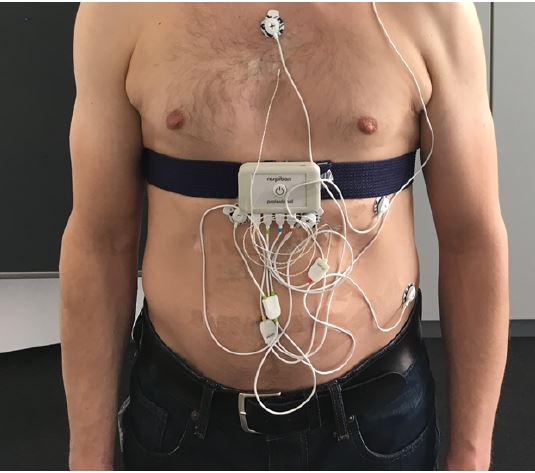
\includegraphics[width=0.45\textwidth]{figures/Posicionamiento pecho wesad.JPG}
        \caption[Posicionamiento de los sensores de pecho en el estudio \textit{WESAD}]
        {Posicionamiento de los sensores de pecho en el estudio \textit{WESAD}. Imagen extraída de \cite{schmidt_introducing_2018}.}
        \label{figure:estado_arte:pecho_wesad}
    \end{figure}

    \begin{figure}[h]
        \centering
        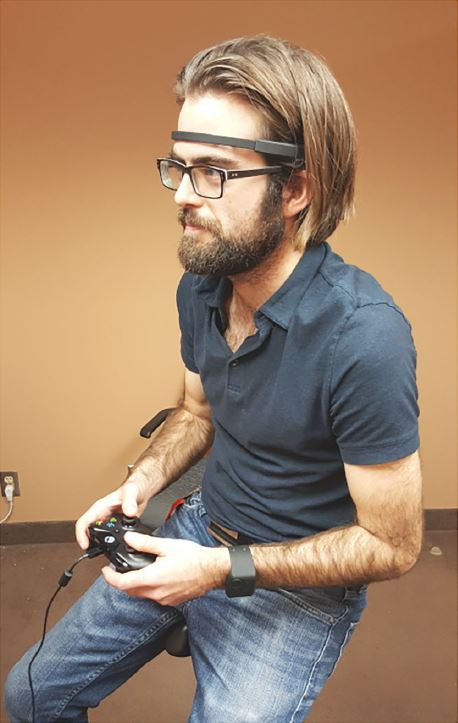
\includegraphics[width=0.33\textwidth]{figures/posiconamiento cabeza pass.JPG}
        \caption[Posicionamiento del sensor de cabeza en el estudio \textit{PASS}]
        {Posicionamiento del sensor de cabeza en el estudio \textit{PASS}. Imagen extraída de \cite{parent_pass_2020}.}
        \label{figure:estado_arte:cabeza_pass}
    \end{figure}

    No obstante, con la publicación de los \glspl{dataset} la comunidad científica puede crear modelos que permitan extraer más información del paciente a partir de estas medidas, mientras que con la progresiva miniaturización y mejora del hardware es posible que en el futuro se puedan extraer datos similares con \glspl{no-invasiva}. Como se detalló en la Sección \ref{section:contexto:wearables}, actualmente es posible encontrar \glspl{wearable}, que si bien de una manera mucho más simple y limitada, permiten realizar pruebas más complejas como los \glspl{ecg} \cite{garcia_electrocardiograma_2024}.

    En segundo lugar, los significativos avances producidos en el ámbito de los \glspl{wearable} permiten mejorar el enfoque visto en la Sección \ref{sec:estado_arte:smartphone} incorporando los datos recogidos por estos sensores. Gracias al \gls{framework} de \textit{Salud Conectada}, es posible abstraerse de la complejidad del hardware, siendo viable leer datos de una gran variedad de dispositivos.
    
    Mientras en \textit{StudentLife} se inferían los ámbitos de sueño mediante la luz y los sonidos capturados por el \gls{smartphone}, con un \gls{wearable} se pueden obtener incluso las fases del sueño del usuario con mayor precisión. En el caso de la movilidad ya no es necesario estimarla mediante GPS o balizas WiFi, es posible obtener directamente la distancia recorrida o los pasos caminados. Análogamente, con el estado del arte actual es practicable el poder leer datos de actividad física más complejos, como las calorías quemadas del usuario o el tipo de ejercicio realizado.

    Por otra parte, en la Sección \ref{sec:estado_arte:apps} se pudo comprobar que la sociedad está consumiendo aplicaciones de salud mental (especialmente, de estrés), estando dispuesta a abonar suscripciones para obtener recomendaciones y consejos. Sin embargo, también se pudo evidenciar que dependen notablemente de los datos suministrados por el usuario, a la vez de sus flaquezas en los ámbitos de privacidad y de rigor científico.

    Por tanto, el valor de la solución propuesta en este \gls{tfm} y planteada en la Sección \ref{sec:objetivos} reside en los siguientes puntos:

    \begin{enumerate}
        \item Explorar las posibilidades de \textit{Salud Conectada} para la obtención de datos de \glspl{wearable}, logrando obtener datos más precisos y fiables con menores costes de desarrollo.
        \item Disponer de cuestionarios y consejos con fundamento científico, los cuales puedan llegar a los usuarios finales. Asimismo, se crea el medio técnico para que investigadores de otras áreas, como la Psicología, puedan desplegar sus experimientos en la realización de pautas y cuestionarios.
        \item A través de este documento y de la publicación del código fuente de todos los componentes del proyecto, aportar mayor transparencia y privacidad para los usuarios en el campo de las aplicaciones de salud mental.
        \item Mediante el diseño del sistema, permitir que futuros proyectos puedan añadir el soporte para leer nuevos datos o conectar de forma sencilla módulos de aprendizaje automático que permitan una mejor estimación del estrés, depresión y/o soledad, o bien profundizar en la construcción de un \gls{dataset} con los datos recopilados que aporte valor a la comunidad científica.
    \end{enumerate}

    Por último se quiere recalcar que esta solución pretende ante todo, mediante el desarrollo de un sistema que pueda ser utilizado en un escenario real, asentar los conceptos teórico/prácticos aprendidos en el Máster. Si bien los aspectos relacionados con la \gls{iss} y el desarrollo de aplicaciones móviles juegan un papel predominante, también se pueden aplicar en menor medida algunos relacionados con otras materias, tales como las redes inalámbricas o los sistemas distribuidos.